%!TEX program = xelatex
\documentclass[dvipsnames, svgnames,a4paper,11pt]{article}
% ----------------------------------------------------
%   中山大学物理与天文学院本科实验报告模板
%   作者:Huanyu Shi,2019级
%   知乎:https://www.zhihu.com/people/za-ran-zhu-fu-liu-xing
%   Github:https://github.com/Huanyu-Shi/SYSU-SPA-Labreport-Template
%   Last update : 2023.4.10
% ----------------------------------------------------

% ----------------------------------------------------- 
%	加边框的命令
%	参考:https://tex.stackexchange.com/questions/531559/how-to-add-the-page-border-for-first-two-pages-in-latex
\usepackage{tikz}
\usetikzlibrary{calc}
\usepackage{eso-pic}
\AddToShipoutPictureBG{%
\begin{tikzpicture}[overlay,remember picture]
\draw[line width=0.6pt] % 边框粗细
    ($ (current page.north west) + (0.6cm,-0.6cm) $)
    rectangle
    ($ (current page.south east) + (-0.6cm,0.6cm) $); % 边框位置
\end{tikzpicture}}


\usepackage{xcolor}
\definecolor{c1}{HTML}{2752C9} % 目录颜色
\definecolor{c2}{RGB}{190,20,83} % 引用颜色

\usepackage{ctex}
\usepackage[top=28mm,bottom=28mm,left=15mm,right=15mm]{geometry}
\usepackage{hyperref} 
\hypersetup{
	colorlinks,
	linktoc = section, % 超链接位置,选项有section, page, all
	linkcolor = c1, % linkcolor 目录颜色
	citecolor = c1  % citecolor 引用颜色
}
\usepackage{amsmath,enumerate,multirow,float}
\usepackage{tabularx}
\usepackage{tabu}
\usepackage{subfig}
\usepackage{fancyhdr}
\usepackage{graphicx}
\usepackage{wrapfig}  
\usepackage{physics}
\usepackage{appendix}
\usepackage{amsfonts}

%
\usepackage{tcolorbox}
\tcbuselibrary{skins,breakable}
\newtcolorbox{tbox}[2][]{
    colframe=black!70!,
    breakable,
    enhanced,
	boxrule =0.5pt,
    title = {#2},
    fonttitle = \large\kaishu\bfseries,
	drop fuzzy shadow,
    #1
}
\newtcolorbox[auto counter,number within=section]{question}[1][]{
  top=2pt,bottom=2pt,arc=1mm,
  boxrule=0.5pt,
%   frame hidden,
  breakable,
  enhanced, %跨页后不会显示下边框
  coltitle=c1!80!gray,
  colframe=c1,
  colback=c1!3!white,
  drop fuzzy shadow,
  title={思考题~\thetcbcounter:\quad},
  fonttitle=\bfseries,
  attach title to upper,
  #1
}
\newcommand{\setLhead}[1]{%
  \lhead{{\color{gray}\kaishu #1}} % 定义新的命令,设置右边页眉的内容
}
\newcommand{\setRhead}[1]{%
  \rhead{{\color{gray}\kaishu #1}} % 定义新的命令,设置右边页眉的内容
}
% ---------------------------------------------------------------------
%	利用cleveref改变引用格式,\cref是引用命令
\usepackage{cleveref}
\crefformat{figure}{#2{\textcolor{c2}{图 #1}}#3} % 图片的引用格式
\crefformat{equation}{#2{(\textcolor{c2}{#1})}#3} % 公式的引用格式
\crefformat{table}{#2{\textcolor{c2}{表 #1}}#3} % 表格的引用格式


% ---------------------------------------------------------------------
%	页眉页脚设置
\fancypagestyle{plain}{\pagestyle{fancy}}
\pagestyle{fancy}
\setLhead{中山大学物理与天文学院基础物理实验预习报告}
%\lhead{\kaishu 中山大学物理与天文学院物理实验\uppercase\expandafter{\romannumeral3}} % 左边页眉,学院 + 课程
%\rhead{{\color{gray}\kaishu Template 实验报告模板}} % 右边页眉,实验报告标题
\setRhead{实验1\hspace{1pt}冰的熔化热测量}
\cfoot{\thepage} % 页脚,中间添加页码


% ---------------------------------------------------------------------
%	对目录、章节标题的设置
\renewcommand{\contentsname}{\centerline{\huge 目录}}
\usepackage{titlesec}
\usepackage{titletoc}
% \titleformat{章节}[形状]{格式}{标题序号}{序号与标题间距}{标题前命令}[标题后命令]
\titleformat{\section}{\centering\LARGE\songti}{}{1em}{}

% ---------------------------------------------------------------------
%   listing代码环境设置
\usepackage{listings}
\lstloadlanguages{python}
\lstdefinestyle{pythonstyle}{
backgroundcolor=\color{gray!5},
language=python,
frameround=tftt,
frame=shadowbox, 
keepspaces=true,
breaklines,
columns=spaceflexible,                   
basicstyle=\ttfamily\small, % 基本文本设置,字体为teletype,大小为scriptsize
keywordstyle=[1]\color{c1}\bfseries, 
keywordstyle=[2]\color{Red!70!black},   
stringstyle=\color{Purple},       
showstringspaces=false,
commentstyle=\ttfamily\scriptsize\color{green!40!black},%注释文本设置,字体为sf,大小为smaller
tabsize=2,
morekeywords={as},
morekeywords=[2]{np, plt, sp},
numbers=left, % 代码行数
numberstyle=\it\tiny\color{gray}, % 代码行数的数字字体设置
stepnumber=1,
rulesepcolor=\color{gray!30!white}
}




% ---------------------------------------------------------------------
%	其他设置
\def\degree{${}^{\circ}$} % 角度
\graphicspath{{./images/}} % 插入图片的相对路径
\allowdisplaybreaks[4]  %允许公式跨页 % 导入模板的相关设置
\usepackage{lipsum}
\usepackage{indentfirst}
\usepackage{pdfpages}
\usepackage{multirow}
\usepackage{subfig}
\usepackage{graphicx}
\usepackage{float} 
\usepackage{booktabs}
\usepackage{enumerate}
\usepackage{makecell} 
\renewcommand{\d}{\mathrm{d}}
\newcommand{\upcite}[1]{\textsuperscript{\textsuperscript{\cite{#1}}}}


%---------------------------------------------------------------------
%	正文
%---------------------------------------------------------------------
\newcommand{\exname}{双光栅测量微弱振动位移量实验}%实验名称
\setRhead{\exname}
\begin{document}


\begin{table}
	\renewcommand\arraystretch{1.7}
	\begin{tabularx}{\textwidth}{
		|X|X|X|X
		|X|X|X|X|}
	\hline
	\multicolumn{2}{|c|}{预习报告}&\multicolumn{2}{|c|}{实验记录}&\multicolumn{2}{|c|}{分析讨论}&\multicolumn{2}{|c|}{总成绩}\\
	\hline
	 \hspace{0.625cm}25& & \hspace{0.625cm}30  & & \hspace{0.625cm}25  & &  \hspace{0.625cm}80 & \\
	\hline
	\end{tabularx}
\end{table}


\begin{table}
	\renewcommand\arraystretch{1.7}
	\begin{tabularx}{\textwidth}{|X|X|X|X|}
	\hline
	专业:& 物理学类 &年级:&2023级 \\
	\hline
	姓名:& 姚昊廷  & 学号:&22322091\\
	\hline
	日期:&2025.3.11 & 教师签名:& \\
	\hline
	\end{tabularx}
\end{table}

\begin{center}
	\LARGE \exname
\end{center}

\textbf{【实验报告注意事项】}
\begin{enumerate}
	\item 实验报告由三部分组成:
	\begin{enumerate}
		\item 预习报告:阅读\underline{\textbf{实验讲义}},弄清实验原理,了解实验需要测量的物理量,完成预习思考题。将预习报告带到实验室并在开始实验前由实验教师或助教检查。预习成绩低于10分(共20分)者不能做实验。
	    \item 实验记录:认真、客观记录实验条件、实验过程中的现象以及数据。实验记录请用珠笔或者钢笔书写并签名(\textcolor{red}{\textbf{用铅笔记录的被认为无效}})。\textcolor{red}{\textbf{保持原始记录,包括写错删除部分。}}离开前请实验教师或助教检查记录并签名。
	    \item 分析讨论:处理实验原始数据,对数据的可靠性和合理性进行分析;按规范呈现数据和结果;分析物理现象(含回答实验思考题,写出思考过程);最后得出结论。
	\end{enumerate}
	\item \underline{\textbf{实验报告}}就是将预习报告、实验记录、和数据处理与分析合起来,加上本页封面。实验记录须手写,预习报告和分析讨论部分手写或打印均可。
	\item 每次完成实验后的一周内交\textbf{实验报告}(特殊情况不能超过两周),每份报告必须注明姓名和学号,合作者和学号,否则按零分处理。
\end{enumerate}



\clearpage
\tableofcontents
\clearpage

\setcounter{section}{0}
\section{\exname\ \textbf{预习报告}}
	
\subsection{实验目的}
\begin{enumerate}
	\item 了解利用光的多普勒频移形成光拍的原理并用于测量光拍拍频 。
	\item 学会使用精确测量微弱振动位移的一种方法 。
	\item 应用双光栅微弱振动测量 仪测量音叉振动的微振幅 。
\end{enumerate}
\subsection{仪器用具}
\begin{table}[htbp]
	\centering
	\renewcommand\arraystretch{1.6}
	% \setlength{\tabcolsep}{10mm}
	\begin{tabular}{p{0.05\textwidth}|p{0.20\textwidth}|p{0.05\textwidth}|p{0.5\textwidth}}
	\hline
	编号& 仪器用具名称 & 数量 &  主要参数(型号,测量范围,测量精度等) \\
	\hline
	1&双光栅微弱振动测量仪&1 &DHGS-1型,半导体激光器:$\lambda$=650nm,功率 2-5mW;音叉谐振频率:500Hz左右。\\
	2&数字示波器&1&DS1000E(D) \\
	3&信号发生器&1 &MFG-2000\\
	\hline
\end{tabular}
\end{table}


\subsection{实验原理概述}
\begin{enumerate}
    \item \textbf{位移光栅的多普勒频移}\par
    多普勒效应是指光源、接收器、传播介质或中间反射器之间的相对运动所引起的接收器
    接收到的光波频率与光源频率发生的变化,由此产生的频率变化称为多普勒频移。

    由于介质对光传播时有不同的相位延迟作用,对于两束相同的单色光,若初始时刻相位
    相同,经过相同的几何路径,但在不同折射率的介质中传播,出射时两光的 位相则不相同,
    对于位相光栅,当激光平面波垂直入射时,由于位相光栅上不同的光密和光疏媒质部分对光
    波的位相延迟作用,使入射的平面波变成出射时的摺 (折 )曲波阵面,见图 1 。
    \begin{figure}[H]
        \centering
        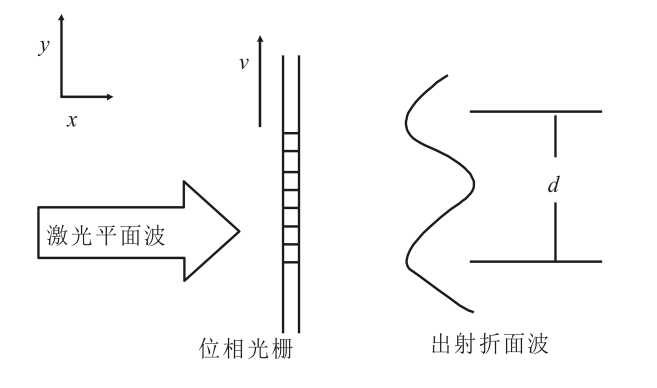
\includegraphics[width=0.8\textwidth]{双光栅1.png}
        \caption{出射的折曲波阵面}
    \end{figure}
    激光平面波垂直入射到光栅,由于光栅上每缝自身的衍射作用和每缝之间的干涉,通过
    光栅后光的强度出现周期性的变化。在远场,我们可以用大家熟知的光栅衍射方程即(1)式
    来表示主极大位置:
    \begin{align}
        d\sin\theta=\pm k\lambda\hspace{2cm}k=0,1,2\cdots
    \end{align}
    式中:整数$k$为主极大级数,$d $为光栅常数,$\theta$ 为衍射角,$\lambda$ 为光波波长。

    如果光栅在$y$方向以速度$v$ 移动,则从光栅出射的光的波阵面也以速度$v$ 在$y$ 方向移动。
    因此在不同时刻,对应于同一级的衍射光射,它从光栅出射时,在$y$ 方向也有一个$vt$ 的位
    移量,见图2。

    这个位移量对应于出射光波位相的变化量为$\Delta \varphi(t)$
    \begin{align}
        \Delta \varphi(t)=\frac{2\pi}{\lambda}\Delta s=\frac{2\pi}{\lambda}vt\sin\theta
    \end{align}
    把(1)代入(2)得:
    \begin{align}
        \Delta \varphi(t)=\frac{2\pi}{\lambda}vt\frac{k\lambda}{d}=k2\pi\frac{v}{d}t=k\omega_d t
    \end{align}
    式中$\omega_d=2\pi\frac{v}{d}$
    \begin{figure}[H]
        \centering
        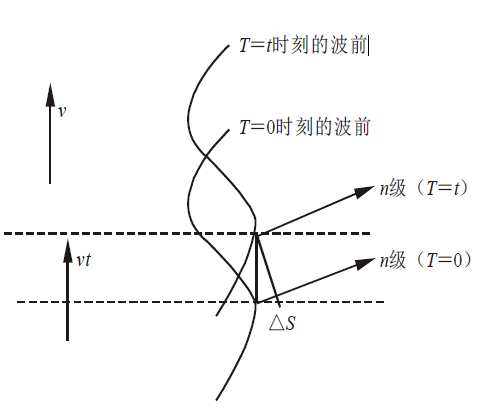
\includegraphics[width=0.8\textwidth]{双光栅2.png}
        \caption{衍射光线在$y$方向上的位移量}
    \end{figure}
    若激光从一静止的光栅出射时;光波电矢量方程为
    \begin{align*}
        E=E_0\cos\omega_0t
    \end{align*}
    而激光从相应移动光栅出射时,光波电矢量方程则为
    \begin{align}
        E=E_0\cos[(\omega_0t+\Delta \varphi(t))]=E_0\cos[(\omega_0+k\omega_d)t]
    \end{align}
    显然可见,移动的位相光栅$k $级衍射光波,相对于静止的位相光栅有一个$\omega_a=\omega_0+k\omega_d$的多普勒频移,如图3 所示。
    \begin{figure}[H]
        \centering
        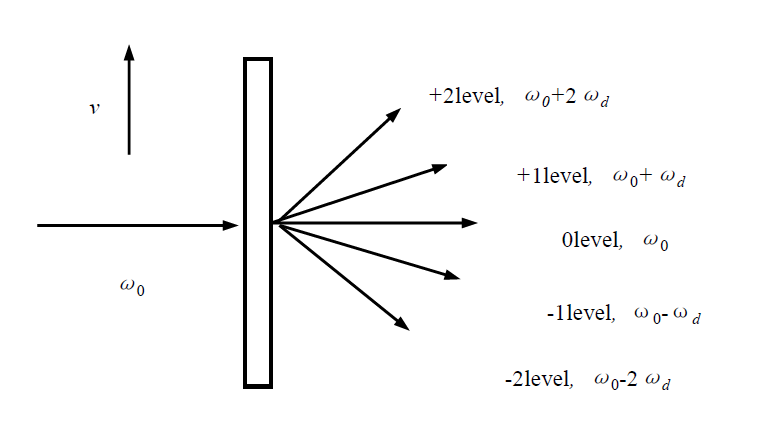
\includegraphics[width=0.8\textwidth]{双光栅3.png}
        \caption{移动光栅的多普勒频移}
    \end{figure}
    \item \textbf{光拍的获得与检测}\par
    光频率很高,为了在光频$\omega_0$中检测出多普勒频移量,必须采用“拍”的方法,即要把
    已频移的和未频移的光束互相平行迭加,以形成光拍。由于拍频较低,容易测得,通过拍频
    即可检测出多普勒频移量。

    本实验形成光拍的方法是采用两片完全相同的光栅平行紧贴,一片B 静止,另一片A
    相对移动。激光通过双光栅后所形成的衍射光,即为两种以上光束的平行迭加,如图4 所示。
    \begin{figure}[H]
        \centering
        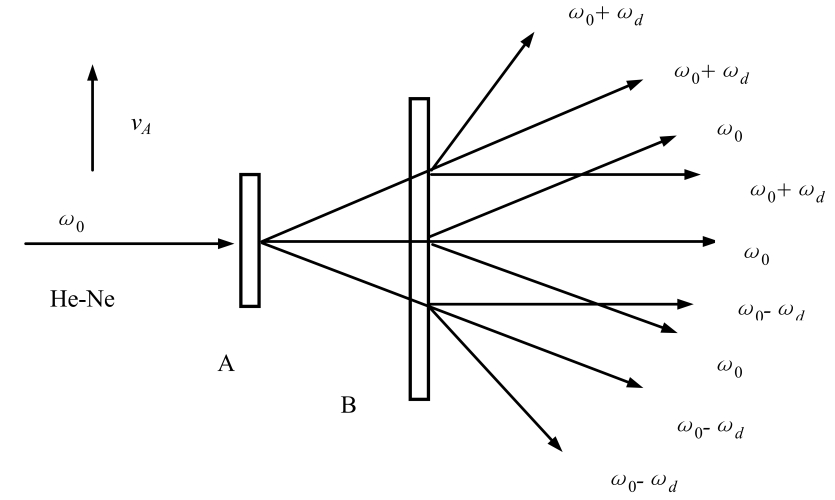
\includegraphics[width=0.8\textwidth]{双光栅4.png}
        \caption{激光通过双光栅后所形成的衍射光}
    \end{figure}
    光栅A 按速度$v_A$移动,起频移作用,而光栅B 静止不动,只起衍射作用,故通过双光
    栅后射出的衍射光包含了两种以上不同频率成分而又平行的光束。由于双光栅紧贴,激光束
    具有一定宽度,故该光束能平行迭加,这样直接而又简单地形成了光拍。如图5 所示。
    \begin{figure}[H]
        \centering
        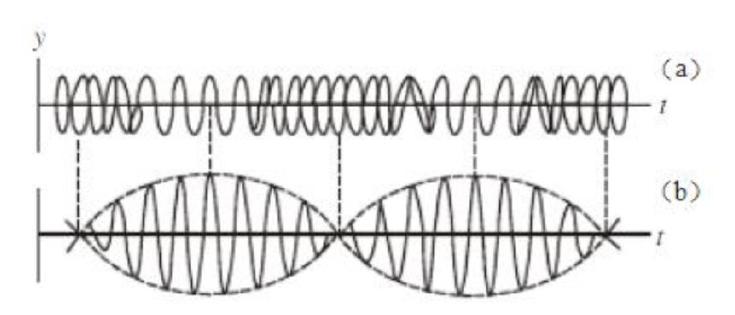
\includegraphics[width=0.8\textwidth]{双光栅5.png}
        \caption{频差较小的两列光波叠加形成“拍”}
    \end{figure}
    当激光经过双光栅所形成的衍射光叠加成光拍信号。光拍信号进入光电检测器后,其输
    出电流可由下述关系求得:
    \begin{equation}
        \begin{aligned}
            \text{光束1:}\hspace{1cm}E_1=E_{10}\cos(\omega_0t+\varphi_1)\\
            \text{光束2:}\hspace{1cm}E_2=E_{20}\cos[(\omega_0+\omega_d)t+\varphi_1]\hspace{1cm}\text{(取k=l)}
        \end{aligned}
    \end{equation}
    光电流:
    \begin{equation}
        \begin{aligned}
            I&=\xi\left(E_{1}+E_{2}\right)^{2} \\
            &=\xi\left\{E_{10}^{2} \cos ^{2}\left(\omega_{0} t+\varphi_{1}\right)+E_{20}^{2} \cos ^{2}\left[\left(\omega_{0}+\omega_{d}\right) t+\varphi_{2}\right]\right. \\
            &+E_{10} E_{20} \cos \left[\left(\omega_{0}+\omega_{d}-\omega_{0}\right) t+\left(\varphi_{2}-\varphi_{1}\right)\right] \\
            &\left.+E_{10} E_{20} \cos \left[\left(\omega_{0}+\omega_{d}+\omega_{0}\right) t+\left(\varphi_{2}+\varphi_{1}\right)\right]\right\}
        \end{aligned}
    \end{equation}
    图中$\xi$为光电转换常数\\
    因光波频率$\omega_0$甚高,在式(6)第一、二、四项中,光电检测器无法反应,式(6)第
    三项即为拍频信号,因为频率较低,光电检测器能做出相应的响应。其光电流为
    \begin{align*}
        i_S=\xi{E_{10}E_{20}\cos[(\omega_0+\omega_d-\omega_0)t+(\varphi_2-\varphi_1)]}=\xi{E_{10}E_{20}\cos[\omega_d t+(\varphi_2-\varphi_1)]}
    \end{align*}
    拍频$F_\text{拍}$即为:
    \begin{align}
        F_\text{拍}=\frac{\omega_d}{2\pi}=\frac{v_A}{d}=v_An_\theta
    \end{align}
    其中$\eta_\theta=\frac{1}{d}$为光栅密度,本实验中$n_\theta=1/d=100\text{条/mm}$
    \item \textbf{微弱振动位移量的检测}\par
    从式(7)可知,$F_\text{拍}$与光频率$\omega_0$无关,且当光栅密度$n_\theta$为常数时,只正比与光栅移动速度$v_A$,如果把光栅粘在音叉上,则$v_A$ 是周期性变化的。所以光拍信号频率$F_\text{拍}$也是随时
    间而变化的,微弱振动的位移振幅为:
    \begin{align}
        A=\frac{1}{2}\int_{0}^{T/2}v(t)\d t=\frac{1}{2}\int_{0}^{T/2}\frac{F_\text{拍}(t)}{n_\theta}\d t=\frac{1}{2n_\theta}\int_{0}^{T/2}F_\text{拍}(t)\d t
    \end{align}
    式中$T$ 为音叉振动周期, $\int_{0}^{T/2}F_\text{拍}(t)\d t$表示$T/2$ 时间内的拍频波的个数,如图6 所示。所
    以,只要测得拍频波的波数,就可得到较弱振动的位移振幅。
    \begin{figure}[H]
        \centering
        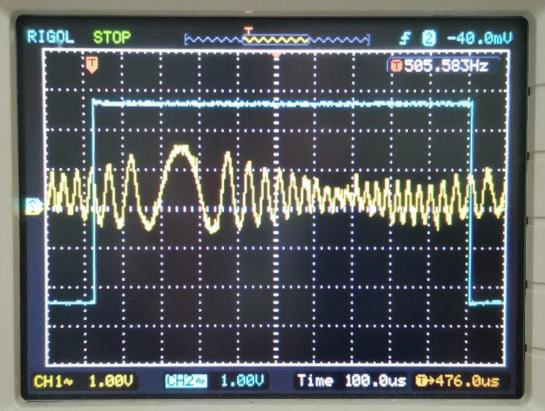
\includegraphics[width=0.8\textwidth]{双光栅6.png}
        \caption{示波器显示$T/2$ 时间内拍频波形(个)数}
    \end{figure} 
    波形数由完整波形数、波的首数、波的尾数三部分组成。根据示波器上显示计算,波形
    的分数部份为不是一个完整波形的首数及尾数,需在波群的两端,可按反正弦函数折算为波
    形的分数部份,即波形数=整数波形数+波的首数和尾数中满1/2 或1/4 或3/4 个波形分数
    部份$+\frac{\sin^{-1}a}{360^\circ}+\frac{\sin^{-1}b}{360^\circ}$
    
    式中a、b 为波群的首、尾幅度和该处完整波形的振幅之比。波群指T/2 内的波形,分
    数波形数若满1/2 个波形为0.5,满1/4 个波形为0.25,满3/4 个波形为0.75。

    如图7,在T/2 内,整数波形数为4,尾数分数部分已满1/4 波形,$b=(H-h)/H=(1-0.6)/1=0.4$。
    所以
    \begin{align*}
        \text{波形数}=4+0.25+\frac{\sin^{-1}0.4}{360^\circ}+\frac{\sin^{-1}23.6^\circ}{360^\circ}=4.25+0.07=4.32
    \end{align*}
    \begin{figure}[H]
        \centering
        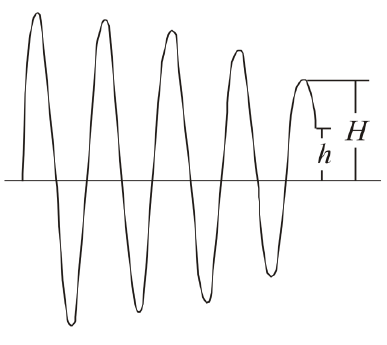
\includegraphics[width=0.8\textwidth]{双光栅7.png}
        \caption{计算波形数}
    \end{figure} 
\end{enumerate}
\subsection{实验前思考题}
\begin{question}
    简述 位移光栅的多普勒频移 原理。
    \tcblower
    当光栅相对于光源或观察者运动时,其周期性结构的运动会调制入射光的相位,导致衍射光的频率发生偏移。这一现象本质上是多普勒效应在周期性结构(光栅)中的体现。
    衍射光的频率偏移量可表示为:
    \begin{align*}
        \Delta f=\frac{mv}{d}
    \end{align*}
    其中$m$为衍射级次,$v$为光栅运动速度,$d$为光栅常数。
\end{question}

\begin{question}
    简述 光拍的获得与检测 方法 和 原理。
    \tcblower
    获得方法:
    \begin{enumerate}
        \item 双频激光干涉法:
        \begin{enumerate}
            \item 方法:使用同一激光源分束为两束光,通过声光调制器(AOM)或电光调制器(EOM)对其中一束进行频率调制,使两束光产生微小频率差($\Delta f$)。
            \item 原理:调制器通过外部信号(如射频驱动)改变光的相位或频率,实现两束光的频率偏移。
        \end{enumerate}
        \item 多普勒频移法
        \begin{enumerate}
            \item 方法:移动反射镜或被测物体,利用多普勒效应改变反射光的频率,与原参考光叠加产生拍频。
            \item 原理:运动导致光程变化,反射光频率偏移($\Delta f = 2v/\lambda$,v为物体速度),与参考光形成差频。
        \end{enumerate}
        \item 双激光器法
        \begin{enumerate}
            \item 方法:使用两个独立激光器,通过温度或电流微调使其频率接近,叠加后产生拍频。
            \item 关键:需稳定激光频率差,避免相位漂移。
        \end{enumerate}
    \end{enumerate}
    光拍的检测方法:
    \begin{enumerate}
        \item 直接光电探测
        \begin{enumerate}
            \item 步骤:两束光经分束器叠加后,由光电探测器(如光电二极管)接收光强信号。
            \item 探测器输出电信号的频率为两束光的频率差($\Delta f $),可用示波器或频谱仪观测。
        \end{enumerate}
        \item 外差检测技术
        \begin{enumerate}
            \item 原理:将光拍频信号与本地振荡器(LO)信号混频,转换为中频信号,便于放大和测量。
            \item 应用:适用于高频(GHz)拍频信号的提取。
        \end{enumerate}
    \end{enumerate}
    形成原理:两束频率相近的光波($f_1$和$f_2$)在空间叠加后,合成光强为:
    \begin{align*}
        I(t)=I_1+I_22\sqrt{I_1I_2}\cos[2\pi(f_1-f_2)t+\Delta \varphi]
    \end{align*}
    其中$f_1-f_2=\Delta f$为拍频频率,$\Delta \varphi$ 为相位差。   
\end{question}

\begin{question}
    简述 微弱振动位移量的检测 方法 和 原理。
    \tcblower
    基于多普勒效应,振动物体反射的激光频率会发生偏移,频移量$\Delta f$与振动速度$v$成正比:
    \begin{align*}
        \Delta f=\frac{2v}{\lambda}
    \end{align*}
    通过积分速度信号可得到位移量。
\end{question}
\clearpage
\setLhead{中山大学物理与天文学院基础物理实验记录}
\begin{table}
	\renewcommand\arraystretch{1.7}
	\centering
	\begin{tabularx}{\textwidth}{|X|X|X|X|}
	\hline
	专业:& 物理学类 &年级:& 2023级 \\
	\hline
	姓名: &姚昊廷& 学号:&22322091  \\
	\hline
	室温:&$22^\circ$C&实验地点:&A505  A4\\
	\hline
	学生签名:& & 评分: &\\
	\hline
	实验时间:& 2025.3.11& 教师签名:&\\
	\hline
	\end{tabularx}
\end{table}
\section{\exname\ \textbf{实验记录}}
\subsection{实验内容、步骤、结果}
\subsubsection{实验内容和步骤}

\subsection{实验过程遇到问题记录}


\clearpage
\setLhead{中山大学物理与天文学院基础物理实验分析与讨论}
\begin{table}
	\renewcommand\arraystretch{1.7}
	\begin{tabularx}{\textwidth}{|X|X|X|X|}
	\hline
	专业:& 物理学 &年级:& 2023级\\
	\hline
	姓名: &姚昊廷& 学号:&22322091 \\
	\hline
    日期:&2025.3.11 &  &\\
	\hline
	评分:&&教师签名:&\\
	\hline
	\end{tabularx}
\end{table}

\section{\exname\ \textbf{分析与讨论}}
\subsection{分析与讨论}

\clearpage
% ---------------------------------------------------------------------
%   参考文献
%   注:使用参考文献时应按照xelatex->bibtex->xelatex->xelatex顺序进行编译
%\phantomsection
%\addcontentsline{toc}{section}{参考文献}
%\bibliographystyle{unsrt}
%\bibliography{myref}
%\begin{thebibliography}{9}
%	\bibitem{ref1} 沈雨欣,翁存程,蒋丽钦.双棱镜干涉法准确测量钠光波长[J].大学物理实验,2023,36(03):40-43.DOI:10.14139/j.cnki.cn22-1228.2023.03.008.
%	\bibitem{ref2} 牟泉润,孙丽媛,杜月棋,等.基于干涉原理的光波长测量装置设计[J].大学物理实验,2021,34(06):80-83+89.DOI:10.14139/j.cnki.cn22-1228.2021.06.018.
%	\bibitem{ref3} 王仁洲,杨涛.一种用激光干涉测量光波波长的新方法[J].大学物理实验,2014,27(06):41-43.DOI:10.14139/j.cnki.cn22-1228.2014.06.014.
%\end{thebibliography}


%\clearpage
\appendix
\appendixpage
\addappheadtotoc
%\subsection*{相图代码}
%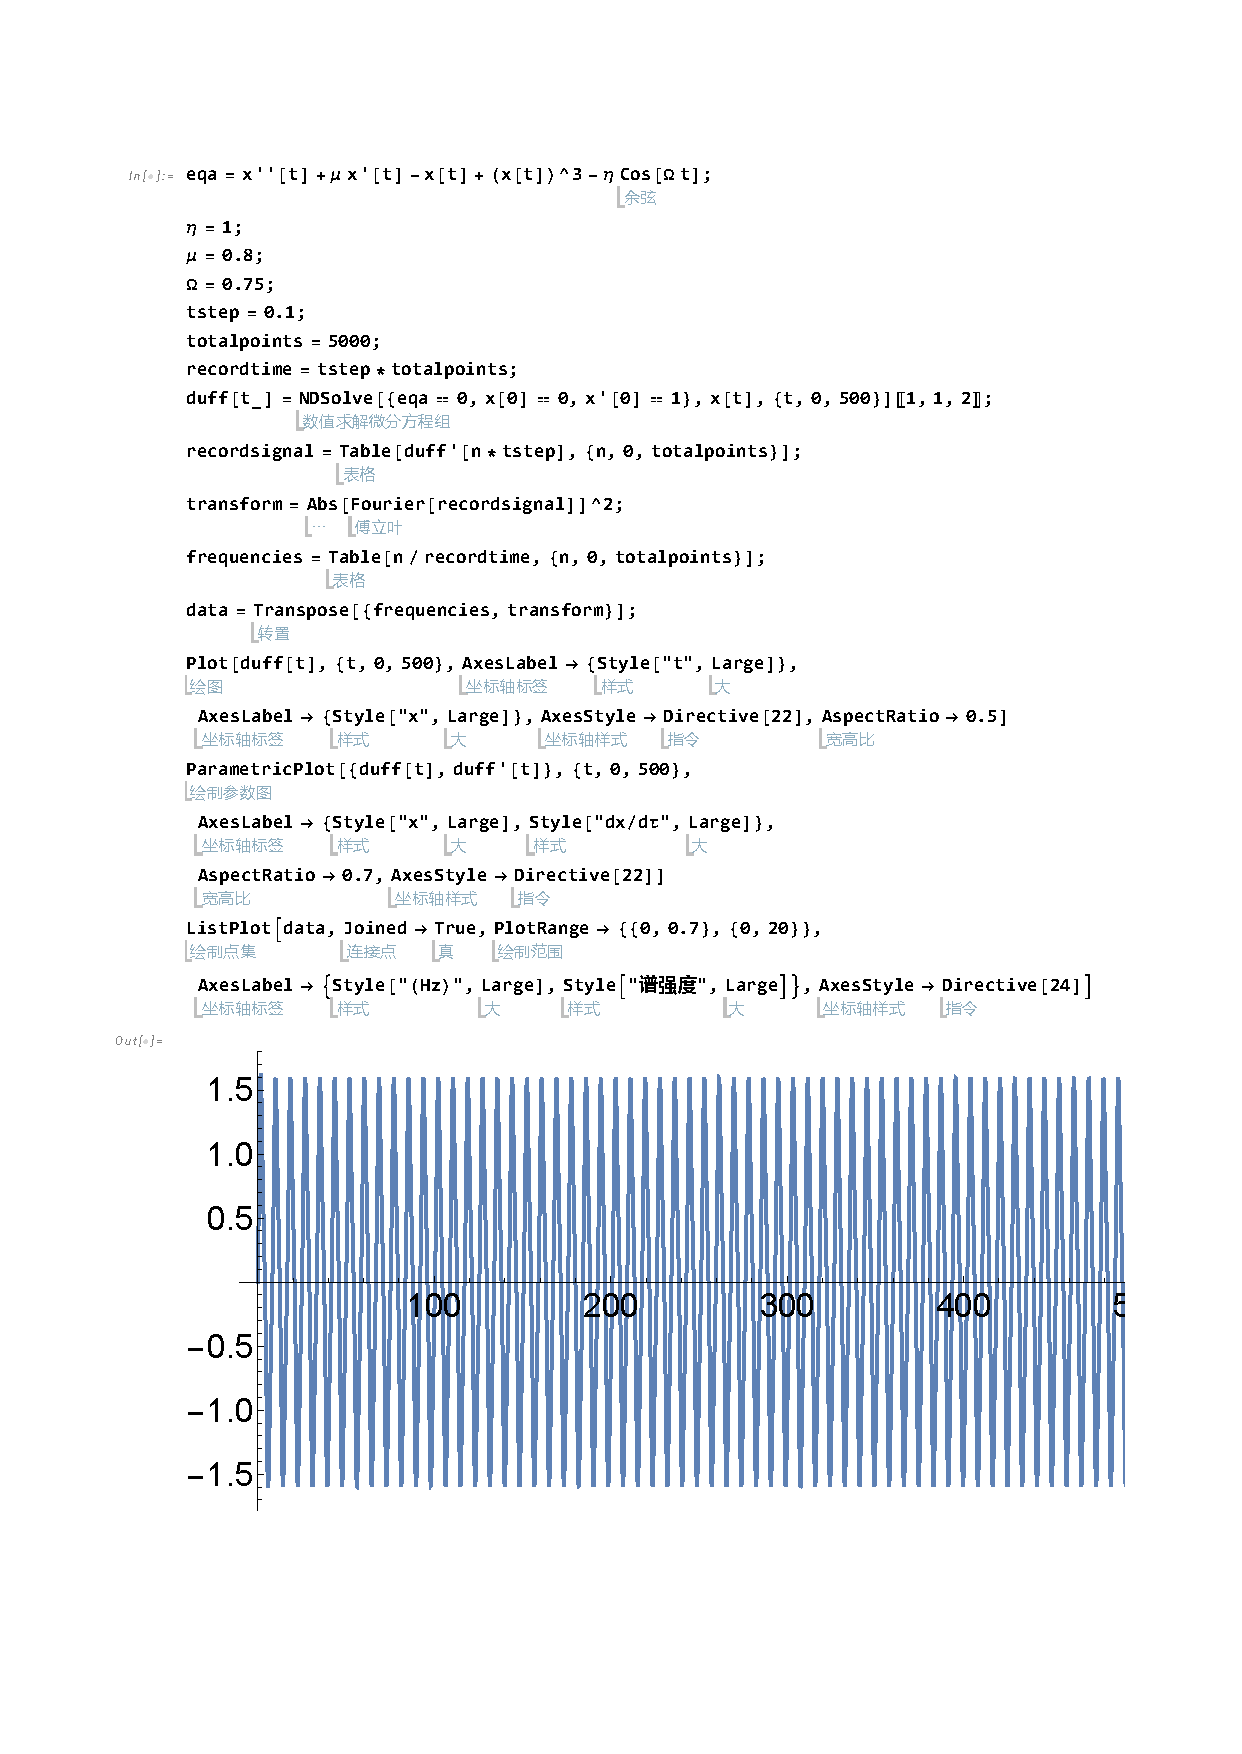
\includepdf[pages=-]{chaos.pdf}
%\subsection*{原件}
%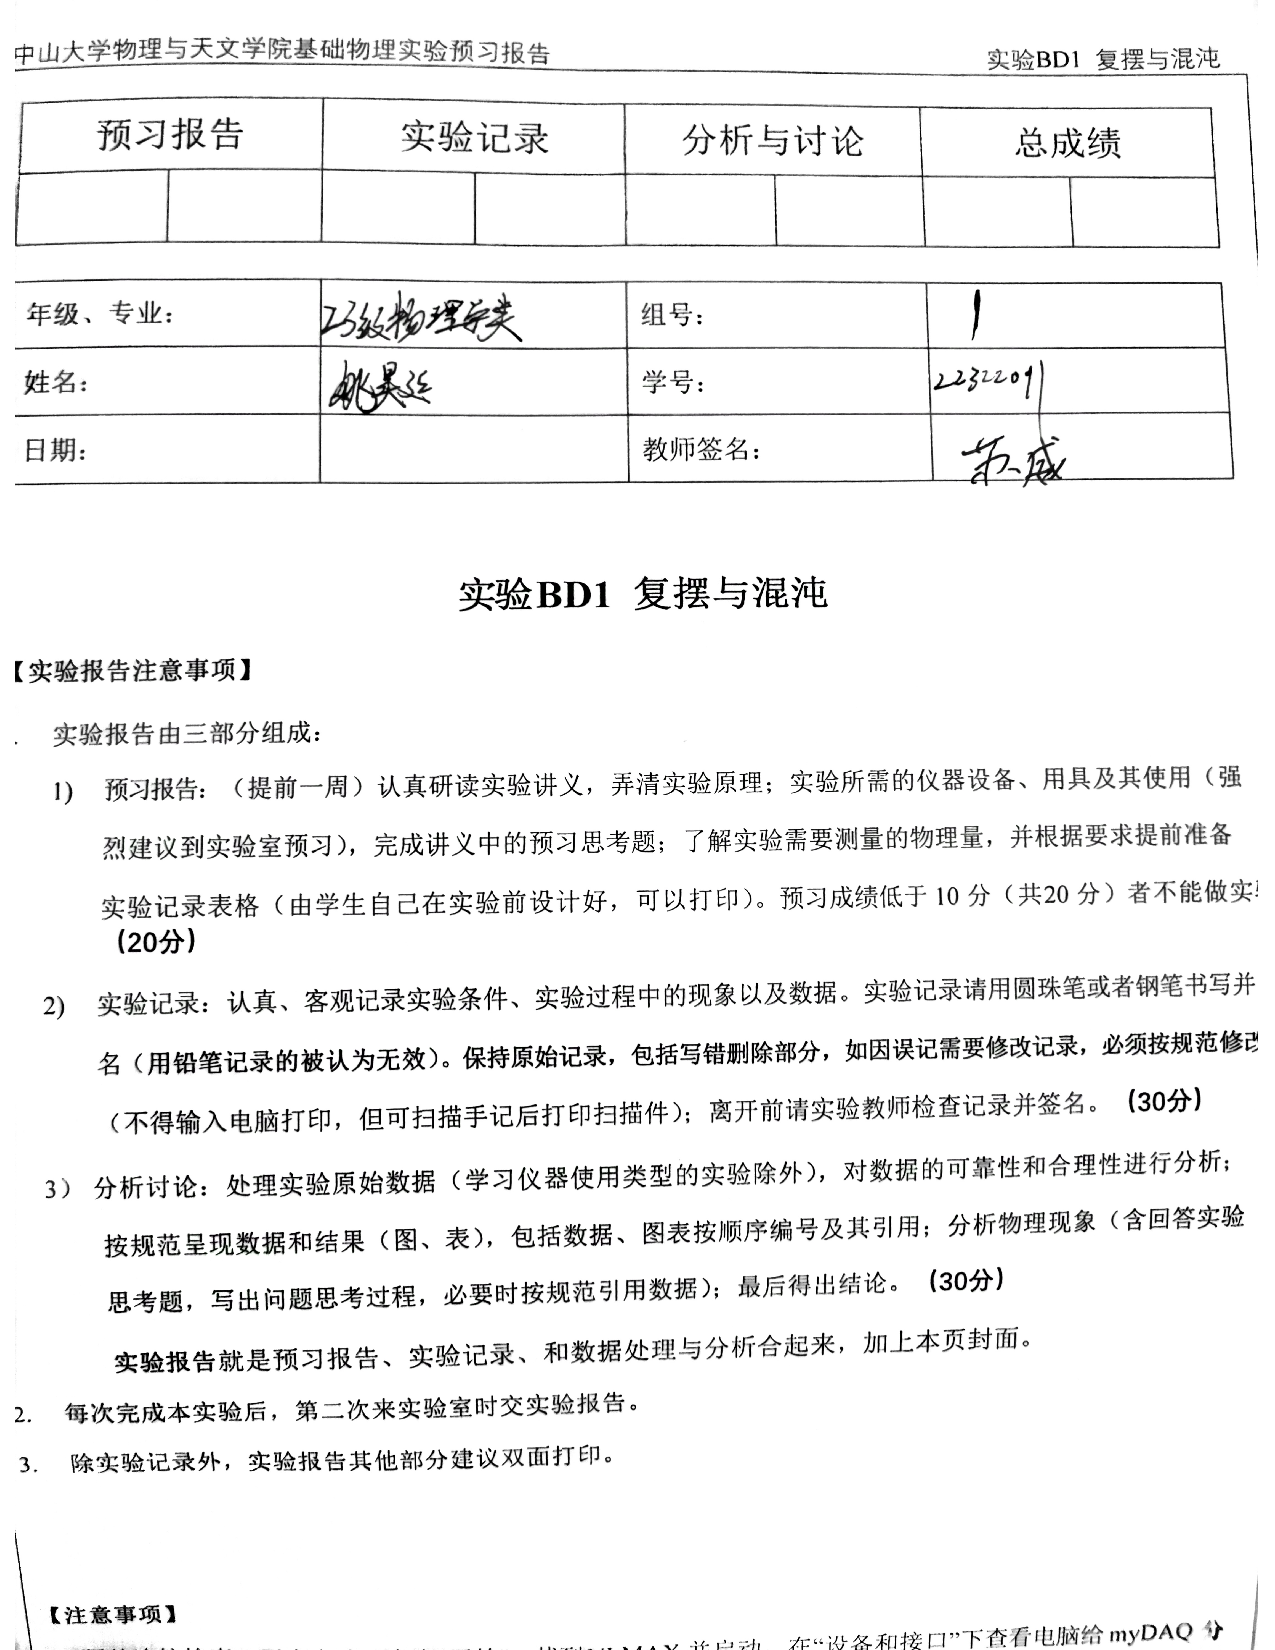
\includepdf[pages=-]{实验3原件.pdf}
%\begin{figure}[H]
%	\centering
%	\includegraphics[width=\textwidth]{焦距数据.jpg}
	
%\end{figure}
%\begin{figure}[H]
%	\centering
%	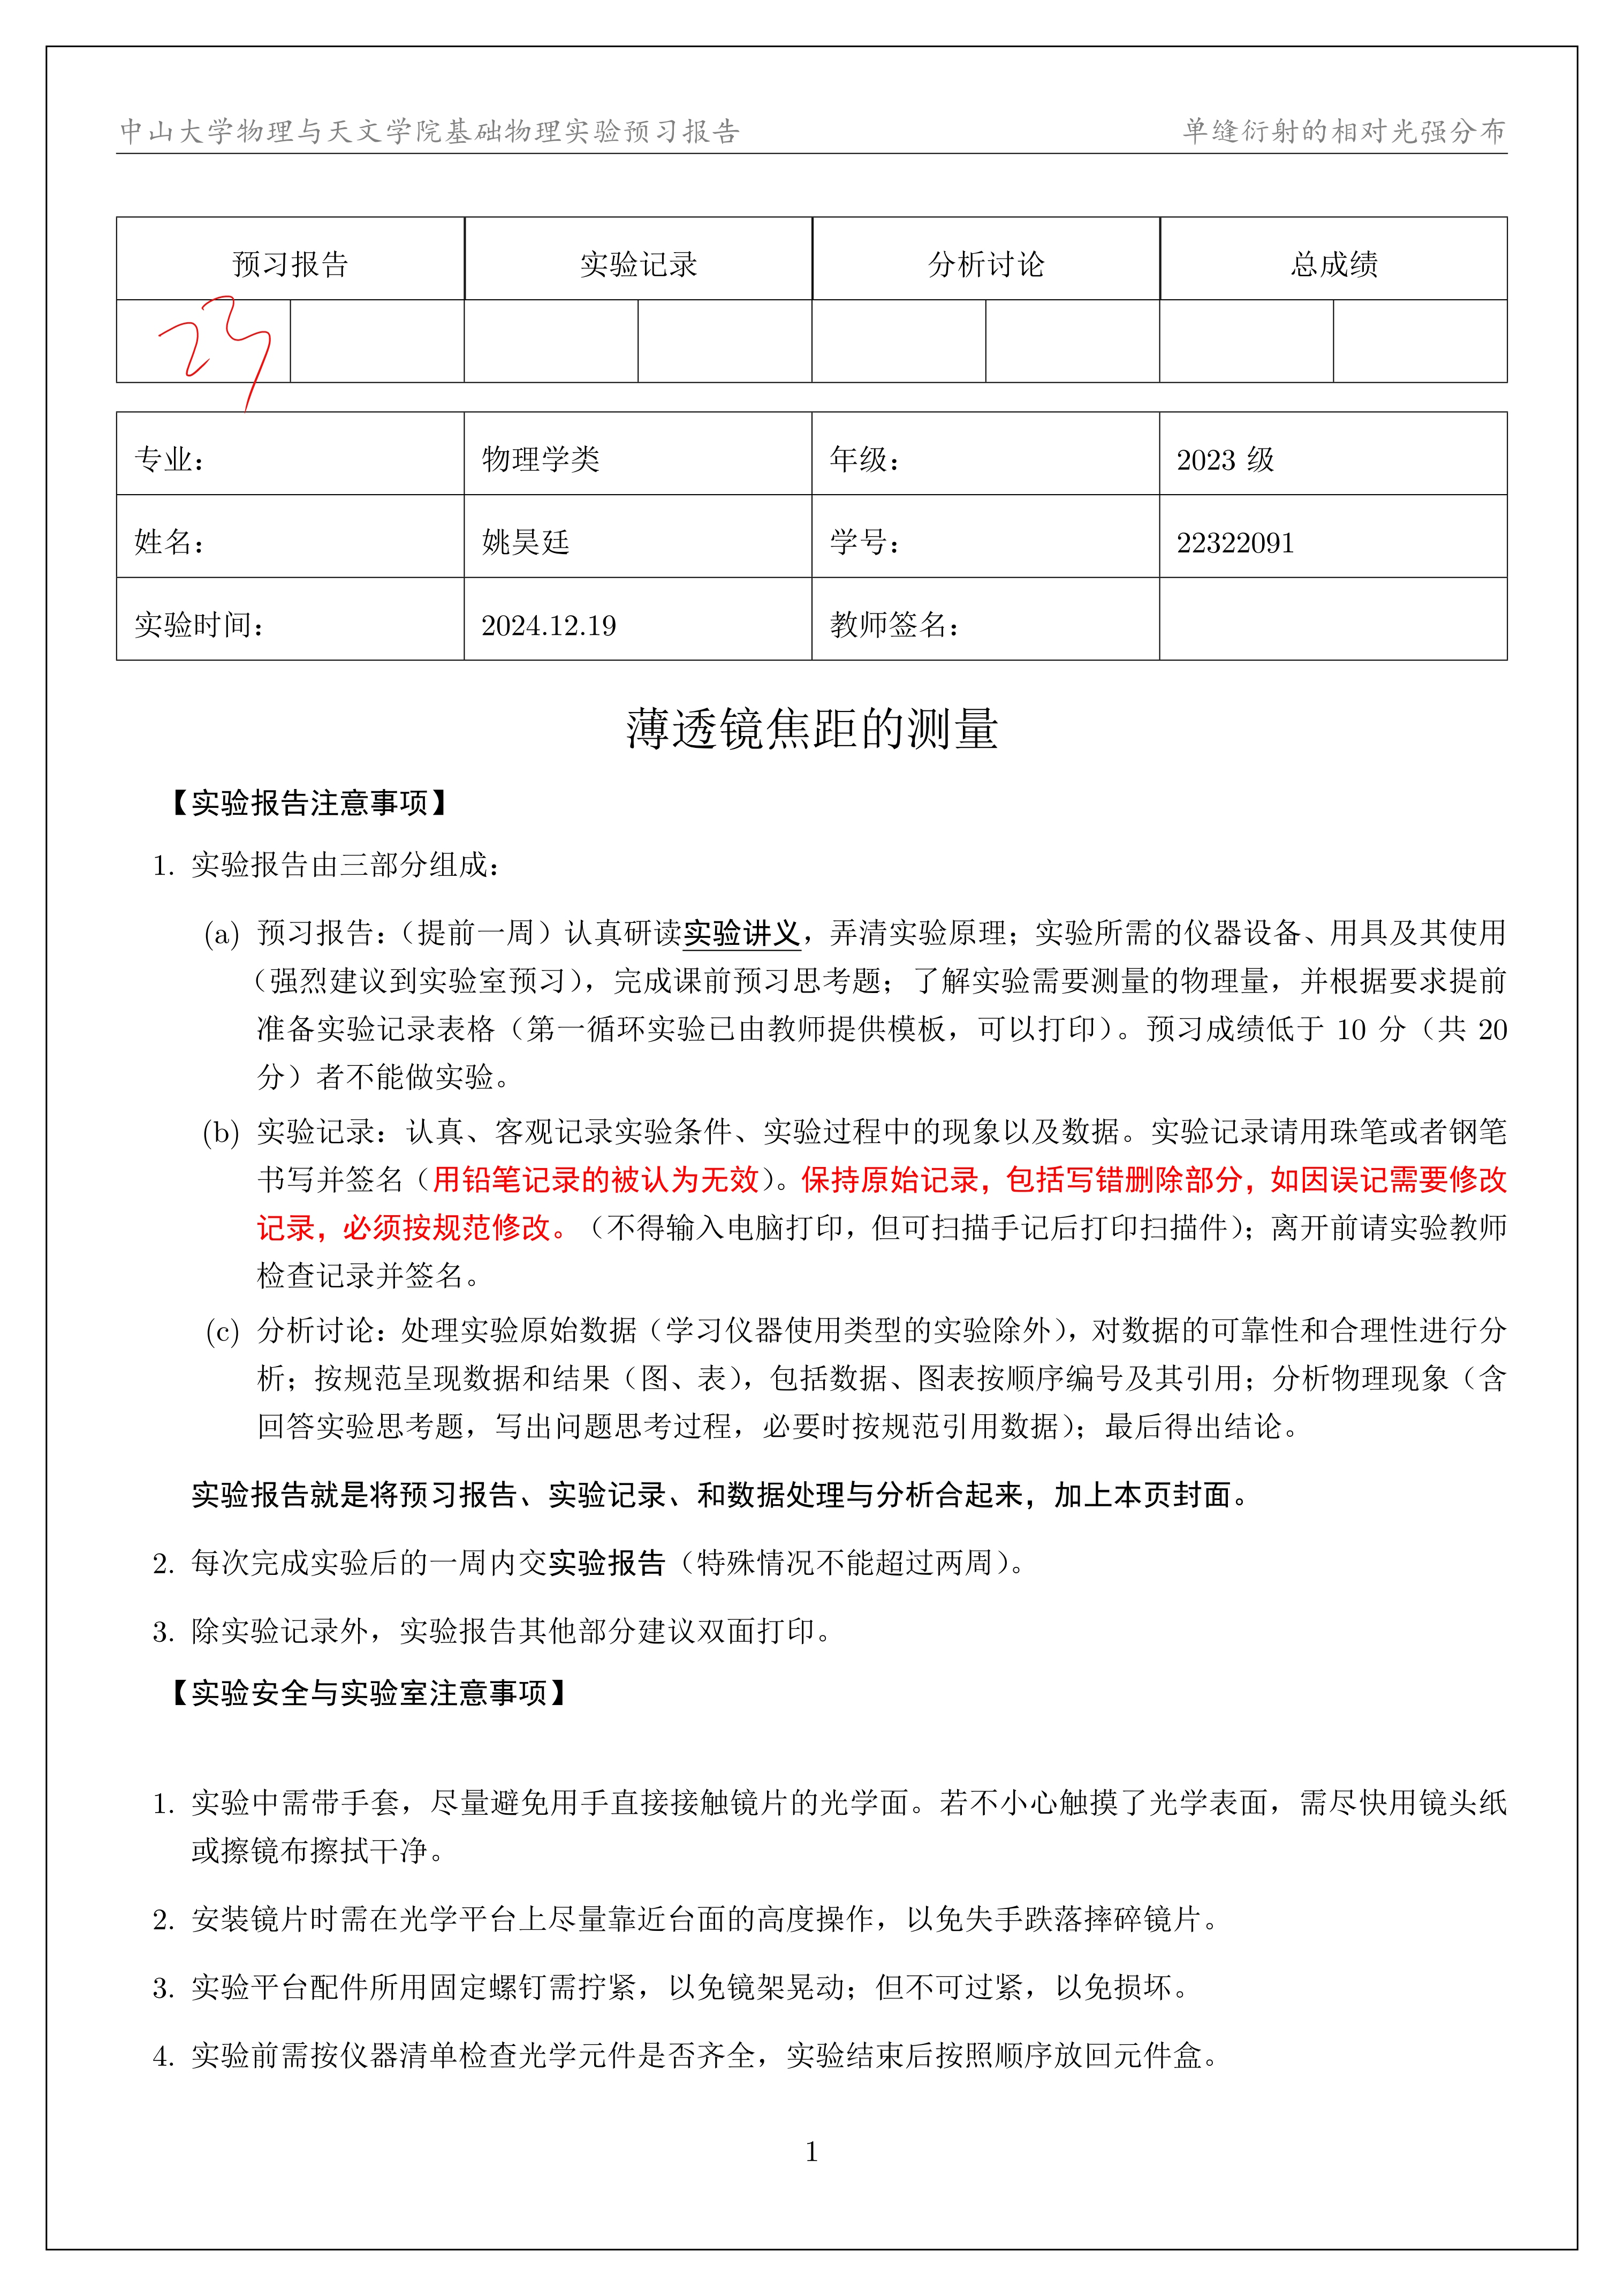
\includegraphics[width=\textwidth]{透镜焦距.jpg}
	
%\end{figure}

%\begin{figure}[H]
%	\centering
%	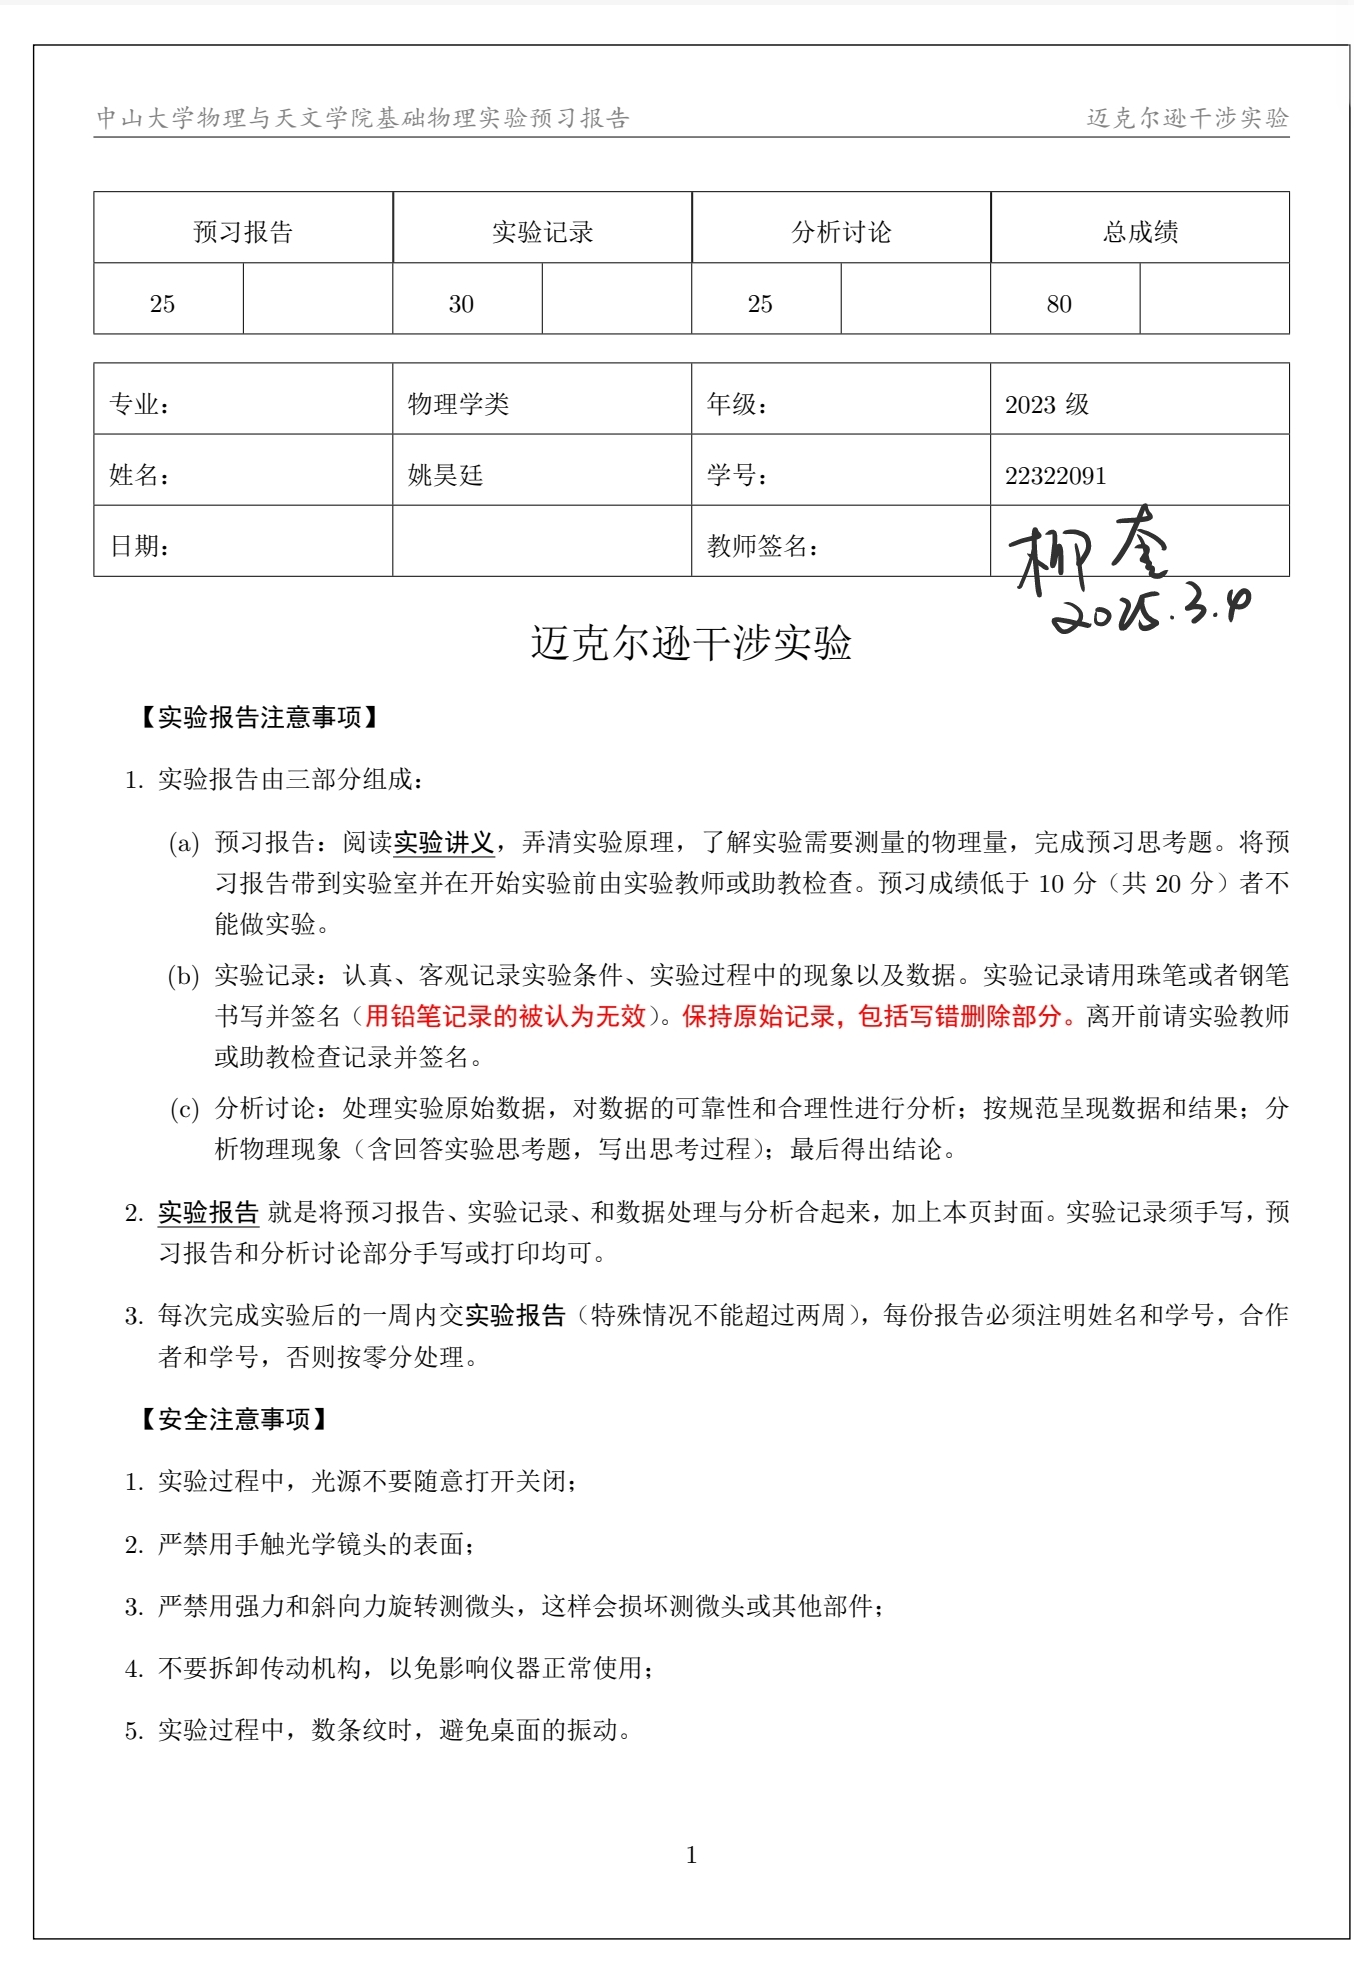
\includegraphics[width=0.4\textwidth]{迈克尔逊原件1.jpg}
%	\includegraphics[width=0.4\textwidth]{迈克尔逊原件2.jpg}
%	\includegraphics[width=0.4\textwidth]{单缝原件3.jpg}
%	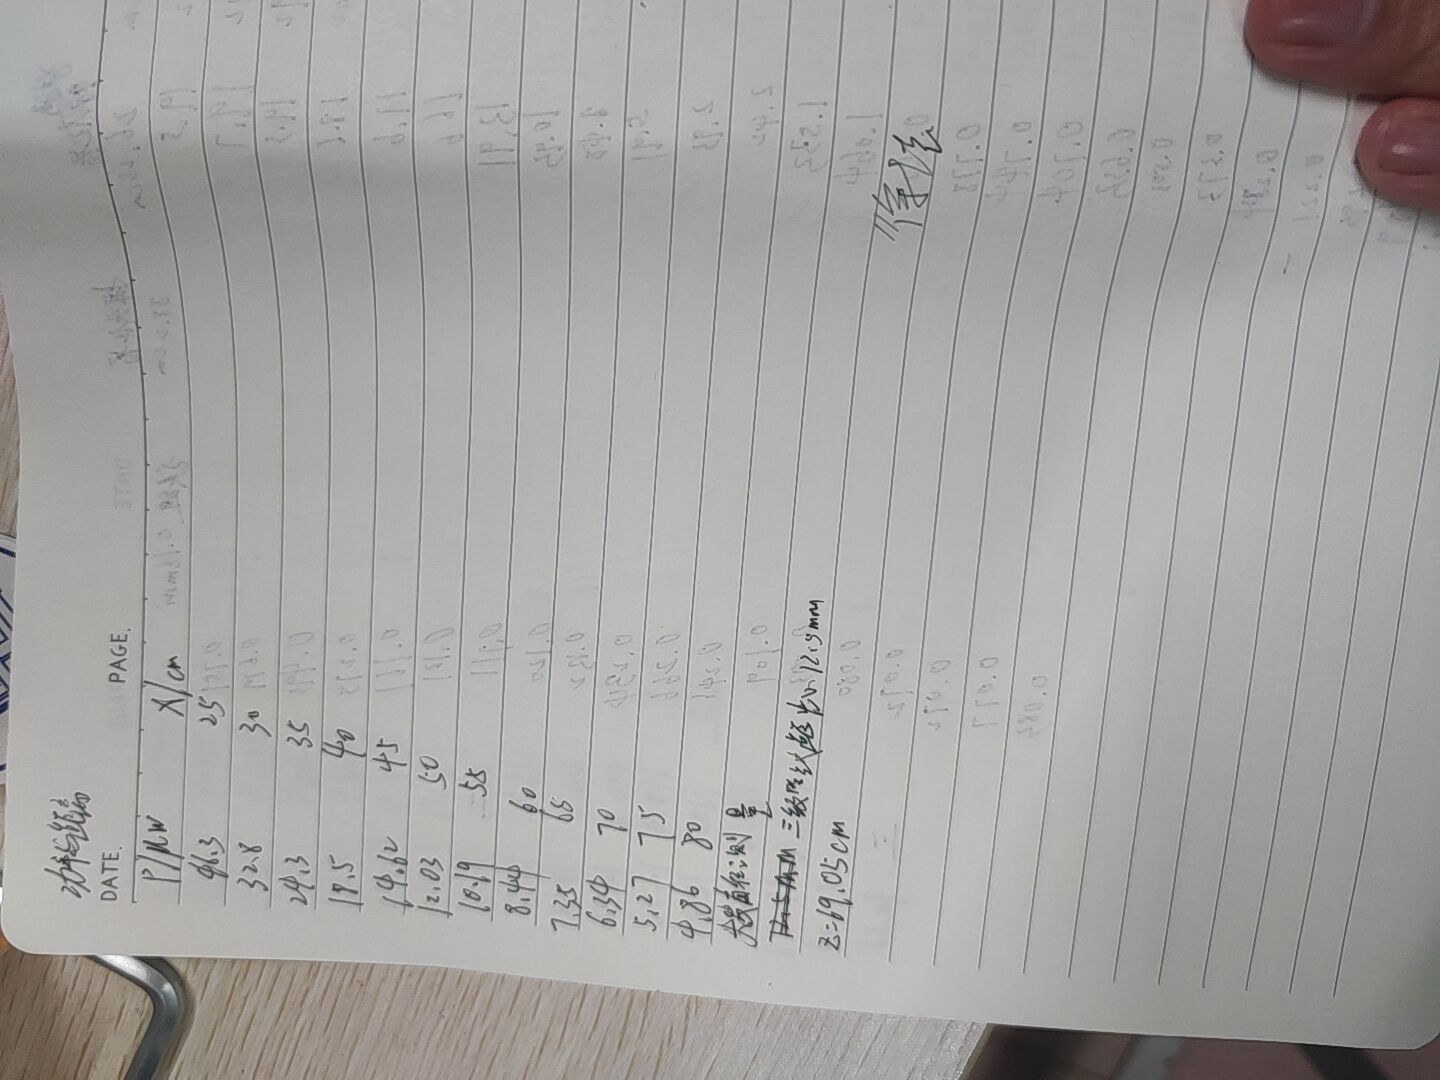
\includegraphics[width=0.4\textwidth]{单缝原件4.jpg}
%\end{figure}
%\subsection*{桌面}
%\begin{figure}[H]
%	\includegraphics[width=0.95\textwidth]{迈克尔逊桌面.jpg}
%\end{figure}
\end{document}
